
Đa phần mọi thứ quanh ta được cấu thành lên từ các nguyên tử và phân tử luôn chuyển động nhiệt không ngừng, giữa các nguyên tử hay phân tử lại có những "liên kết" với nguồn gốc là những lực cơ bản. Những liên kết này đóng vai trò là cấu nối tương tác, duy trình sự ổn định của vật liệu với một nguồn năng lượng tiềm tàng ẩn trong các tương tác đó.

\begin{figure}[!ht]
    \centering
    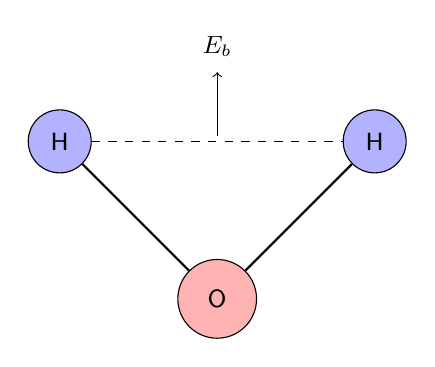
\begin{tikzpicture}[scale=2, font=\sansmath\sffamily, every node/.style={font=\sansmath\sffamily\small}]

% Nguyên tử Oxy
\node[circle, draw, fill=red!30, minimum size=1cm] (O) at (0,0) {O};

% Nguyên tử Hydro
\node[circle, draw, fill=blue!30, minimum size=0.8cm] (H1) at (-1,1) {H};
\node[circle, draw, fill=blue!30, minimum size=0.8cm] (H2) at (1,1) {H};

% Các liên kết
\draw[thick] (O) -- (H1);
\draw[thick] (O) -- (H2);

% Đường gạch giữa hai nguyên tử Hydro
\draw[dashed] (H1) -- (H2);

% Ghi chú E_b
\node (Eb) at (0,1.6) {$E_b$};

% Mũi tên nhỏ từ đường gạch lên E_b
\draw[->, shorten >=2pt, shorten <=2pt] (0,1) -- (Eb);

\end{tikzpicture}
    \caption{Lực liên kết}
\end{figure}


Đối với các vật rắn, những nguyên tử dao động quanh vị trí cân bằng, sắp xếp chặt chẽ với nhau tạo thành một cấu trúc tương đối ổn định. Tuyệt đại đa số chất rắn trong thiên nhiên lại có cấu trúc tinh thể--nguyên tử được sắp xếp trật tự đều đặn và lặp lại tuần hoàn. Cấu trúc tinh thể lại được phân làm nhiều loại phụ thuộc vào đặc điểm hình học của từng hệ.
Ta sẽ khảo sát thuỷ tinh silica--một vật liệu có cấu trúc đó trong bài toán.
\vspace{8pt}

Khi một vật bị phá vỡ, rất nhiều các liên kết phân tử bị đứt gãy và năng lượng liên kết được giải phóng dưới dạng nhiệt và sóng âm. Sau đây, ta sẽ xem xét tỉ lệ phần trăm tổng năng lượng nhận được được sử dụng trục tiếp vào việc bẻ gãy các liên kết phân tử. \footnote{ Năng lượng cần thiết để bẻ gãy liên kểt gọi là năng lượng liên kết, ký hiệu $E_b$.}
\vspace{8pt}

Chú ý rằng, trong nhiều vật liệu, liên kết giữa hai phân tử giảm rất mạnh theo khoảng cách và thường chỉ đáng kể đối với hai phân tử liền kề. Do vậy, ta sẽ chỉ xét năng lượng liên kết của hai phân tử liền kề nhau trong khuôn khổ bài toán.
\vspace{8pt}
 
Ngoài ra, trong phần này ta chỉ quan tâm đến cỡ độ lớn của các đại lượng, các con số được tính ra với những các ước lượng khác nhau có thể sai lệch một khoảng không quá lớn.

\subsection*{Hệ lập phương}
 
Một mô hình đơn giản là thuỷ tinh có cấu trúc mạng lập phương. Điều đó có nghĩa là mỗi phân tử $\mathrm{SiO_2}$, được coi như các quả cầu, chỉ nằm trong một hình lập phương có cạnh dài $2r$, với $r$ là bán kính phân tử. Một ô lập phương như vậy gọi là một \textbf{ô mạng cơ sở}.
\vspace{8pt}

\textbf{Ô đơn vị} (xem \figref{P2_I1}) là ô hình học mà bằng cách lặp đi lặp lại việc tịnh tiến một ô như vậy ta có thể tạo thành cả mạng tinh thể. Cần chú ý rằng hệ tinh thể không có các nguyên tử trong các ô đơn vị, nó chỉ là những biểu diễn hình học mà thôi.\footnote{ Có tất cả bảy hệ tinh thể.}
\vspace{8pt}

\begin{figure}[!ht]
    \centering
    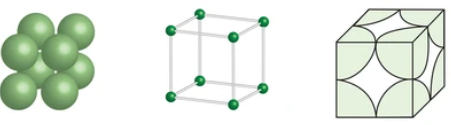
\includegraphics[width=0.7\linewidth]{Problem_2/Image/P2_I1.png}
    \caption{Cấu trúc lập phương}
    \label{P2_I1}
\end{figure}

\Figref{P2_tikz2} trình bày hình ảnh mặt cắt ngang của một phần trong mạng tinh thể, các hình tròn là các phân tử nằm trong các hình vuông là ô cơ sở. Ô đơn vị là những hình vuông nằm giữa các phân tử mà trên \figref{P2_tikz2} là các hình vuông với đỉnh nằm ở tâm bốn hình tròn gần nhau. 
\begin{figure}[!ht]
\centering

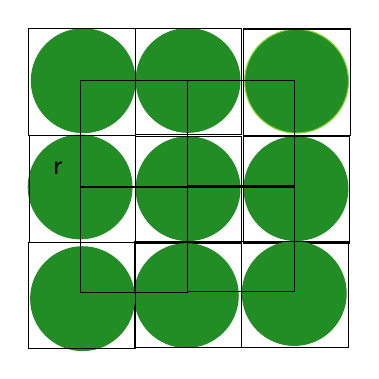
\begin{tikzpicture}[font=\sansmath\sffamily, x=0.75pt,y=0.75pt,yscale=-1,xscale=1]
%uncomment if require: \path (0,347); %set diagram left start at 0, and has height of 347

%Shape: Circle [id:dp09528747501265789] 
\draw  [color={rgb, 255:red, 34; green, 141; blue, 36 }  ,draw opacity=1 ][fill={rgb, 255:red, 34; green, 141; blue, 36 }  ,fill opacity=1 ] (337.33,165.33) .. controls (337.33,151.53) and (348.53,140.33) .. (362.33,140.33) .. controls (376.14,140.33) and (387.33,151.53) .. (387.33,165.33) .. controls (387.33,179.14) and (376.14,190.33) .. (362.33,190.33) .. controls (348.53,190.33) and (337.33,179.14) .. (337.33,165.33) -- cycle ;
%Shape: Square [id:dp5549834318221732] 
\draw   (336.93,140.2) -- (388.27,140.2) -- (388.27,191.53) -- (336.93,191.53) -- cycle ;
%Shape: Circle [id:dp254649691962442] 
\draw  [color={rgb, 255:red, 34; green, 141; blue, 36 }  ,draw opacity=1 ][fill={rgb, 255:red, 34; green, 141; blue, 36 }  ,fill opacity=1 ] (389.33,165.33) .. controls (389.33,151.53) and (400.53,140.33) .. (414.33,140.33) .. controls (428.14,140.33) and (439.33,151.53) .. (439.33,165.33) .. controls (439.33,179.14) and (428.14,190.33) .. (414.33,190.33) .. controls (400.53,190.33) and (389.33,179.14) .. (389.33,165.33) -- cycle ;
%Shape: Square [id:dp7521712816533537] 
\draw   (388.93,140.2) -- (440.27,140.2) -- (440.27,191.53) -- (388.93,191.53) -- cycle ;
%Shape: Circle [id:dp31352442918501755] 
\draw  [color={rgb, 255:red, 34; green, 141; blue, 36 }  ,draw opacity=1 ][fill={rgb, 255:red, 34; green, 141; blue, 36 }  ,fill opacity=1 ] (285.33,164.5) .. controls (285.33,150.69) and (296.53,139.5) .. (310.33,139.5) .. controls (324.14,139.5) and (335.33,150.69) .. (335.33,164.5) .. controls (335.33,178.31) and (324.14,189.5) .. (310.33,189.5) .. controls (296.53,189.5) and (285.33,178.31) .. (285.33,164.5) -- cycle ;
%Shape: Square [id:dp5215635546556922] 
\draw   (285.83,139.8) -- (337.17,139.8) -- (337.17,191.13) -- (285.83,191.13) -- cycle ;
%Shape: Circle [id:dp8519227919361114] 
\draw  [color={rgb, 255:red, 34; green, 141; blue, 36 }  ,draw opacity=1 ][fill={rgb, 255:red, 34; green, 141; blue, 36 }  ,fill opacity=1 ] (336.5,216.83) .. controls (336.5,203.03) and (347.69,191.83) .. (361.5,191.83) .. controls (375.31,191.83) and (386.5,203.03) .. (386.5,216.83) .. controls (386.5,230.64) and (375.31,241.83) .. (361.5,241.83) .. controls (347.69,241.83) and (336.5,230.64) .. (336.5,216.83) -- cycle ;
%Shape: Square [id:dp3236232559839335] 
\draw   (336.6,190.7) -- (387.93,190.7) -- (387.93,242.03) -- (336.6,242.03) -- cycle ;
%Shape: Circle [id:dp948966870385968] 
\draw  [color={rgb, 255:red, 34; green, 141; blue, 36 }  ,draw opacity=1 ][fill={rgb, 255:red, 34; green, 141; blue, 36 }  ,fill opacity=1 ] (337.33,113.17) .. controls (337.33,99.36) and (348.53,88.17) .. (362.33,88.17) .. controls (376.14,88.17) and (387.33,99.36) .. (387.33,113.17) .. controls (387.33,126.97) and (376.14,138.17) .. (362.33,138.17) .. controls (348.53,138.17) and (337.33,126.97) .. (337.33,113.17) -- cycle ;
%Shape: Square [id:dp7704640056265294] 
\draw   (336.93,88.03) -- (388.27,88.03) -- (388.27,139.37) -- (336.93,139.37) -- cycle ;
%Shape: Circle [id:dp21750961656288648] 
\draw  [color={rgb, 255:red, 34; green, 141; blue, 36 }  ,draw opacity=1 ][fill={rgb, 255:red, 34; green, 141; blue, 36 }  ,fill opacity=1 ] (286.83,113.33) .. controls (286.83,99.53) and (298.03,88.33) .. (311.83,88.33) .. controls (325.64,88.33) and (336.83,99.53) .. (336.83,113.33) .. controls (336.83,127.14) and (325.64,138.33) .. (311.83,138.33) .. controls (298.03,138.33) and (286.83,127.14) .. (286.83,113.33) -- cycle ;
%Shape: Square [id:dp023375777050106628] 
\draw   (285.53,88.2) -- (336.87,88.2) -- (336.87,139.53) -- (285.53,139.53) -- cycle ;
%Shape: Circle [id:dp08410780423004927] 
\draw  [color={rgb, 255:red, 126; green, 211; blue, 33 }  ,draw opacity=1 ][fill={rgb, 255:red, 34; green, 141; blue, 36 }  ,fill opacity=1 ] (389.63,113.53) .. controls (389.63,99.73) and (400.83,88.53) .. (414.63,88.53) .. controls (428.44,88.53) and (439.63,99.73) .. (439.63,113.53) .. controls (439.63,127.34) and (428.44,138.53) .. (414.63,138.53) .. controls (400.83,138.53) and (389.63,127.34) .. (389.63,113.53) -- cycle ;
%Shape: Square [id:dp4096382997581849] 
\draw   (389.23,88.4) -- (440.57,88.4) -- (440.57,139.73) -- (389.23,139.73) -- cycle ;
%Shape: Circle [id:dp2759735468682599] 
\draw  [color={rgb, 255:red, 34; green, 141; blue, 36 }  ,draw opacity=1 ][fill={rgb, 255:red, 34; green, 141; blue, 36 }  ,fill opacity=1 ] (286.5,218.33) .. controls (286.5,204.53) and (297.69,193.33) .. (311.5,193.33) .. controls (325.31,193.33) and (336.5,204.53) .. (336.5,218.33) .. controls (336.5,232.14) and (325.31,243.33) .. (311.5,243.33) .. controls (297.69,243.33) and (286.5,232.14) .. (286.5,218.33) -- cycle ;
%Shape: Square [id:dp8215492752117758] 
\draw   (285.6,191.2) -- (336.93,191.2) -- (336.93,242.53) -- (285.6,242.53) -- cycle ;
%Shape: Circle [id:dp09537557723600643] 
\draw  [color={rgb, 255:red, 34; green, 141; blue, 36 }  ,draw opacity=1 ][fill={rgb, 255:red, 34; green, 141; blue, 36 }  ,fill opacity=1 ] (388.5,215.83) .. controls (388.5,202.03) and (399.69,190.83) .. (413.5,190.83) .. controls (427.31,190.83) and (438.5,202.03) .. (438.5,215.83) .. controls (438.5,229.64) and (427.31,240.83) .. (413.5,240.83) .. controls (399.69,240.83) and (388.5,229.64) .. (388.5,215.83) -- cycle ;
%Shape: Square [id:dp6889139441622811] 
\draw   (388.1,190.7) -- (439.43,190.7) -- (439.43,242.03) -- (388.1,242.03) -- cycle ;
%Shape: Square [id:dp8182120104489065] 
\draw   (310.6,113.2) -- (361.93,113.2) -- (361.93,164.53) -- (310.6,164.53) -- cycle ;
%Shape: Square [id:dp9870127822168651] 
\draw   (362.1,113.2) -- (413.43,113.2) -- (413.43,164.53) -- (362.1,164.53) -- cycle ;
%Shape: Square [id:dp4726375642600965] 
\draw   (310.6,164.2) -- (361.93,164.2) -- (361.93,215.53) -- (310.6,215.53) -- cycle ;
%Shape: Square [id:dp991370682204621] 
\draw   (362.1,163.7) -- (413.43,163.7) -- (413.43,215.03) -- (362.1,215.03) -- cycle ;

% Text Node
\draw (303.16,155.64) node   [align=left] {\begin{minipage}[lt]{8.67pt}\setlength\topsep{0pt}
r
\end{minipage}};


\end{tikzpicture}

\caption{Mặt cắt ngang của một phần trong mạng tinh thể}
\label{P2_tikz2}
\end{figure}


\vspace{8pt}

\newpage

\Figref{P2_I2} dưới đây cho thấy một mảnh kính có chiều dài $a$, chiều rộng $b$ và chiều cao $c$ được nhìn từ trên xuống, với $a=75\,\mathrm{mm},\ b=25\,\mathrm{mm},\ c=1\,\mathrm{mm}$ và mỗi ô li có chiều dài $1\,\mathrm{mm}$. Mảnh kính được thả rơi từ độ cao $h=1\,\mathrm{m}$ và vỡ thành $4$ mảnh.

\begin{figure}[!ht]
    \centering
    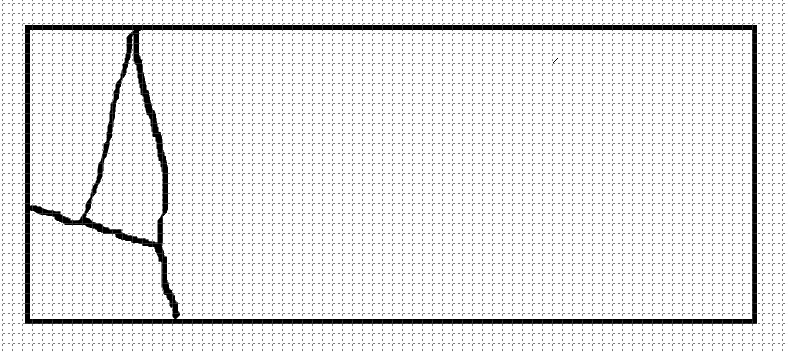
\includegraphics[width=0.8\linewidth]{Problem_2/Image/P2_I2.png}
    \caption{Mảnh kính vỡ}
    \label{P2_I2}
\end{figure}
\vspace{8pt}

\begin{enumerate}[label=(\alph*)]
    \item Sử dụng \figref{P2_I2}, đánh giá gần đúng tổng chiều dài rãnh gãy và tổng số liên kết bị gãy.
    \item Sử dụng ẩn nhiệt hoá hơi của thuỷ tinh, hãy ước tính năng lượng liên kết của thuỷ tinh.
\underline{\textbf{Gợi ý:}} Chứng minh rằng nếu số phân tử mà một phân tử tiếp xúc là $A$ thì số liên kết có trong $n$ phân tử là $An/2$, biết rằng $n$ là rất lớn.
    \item Có bao nhiêu phần trăm năng lượng va chạm được dùng để bẻ gãy các liên kết?
\end{enumerate}

\newpage
\textbf{\underline{Áp dụng số}}
\begin{itemize}
    \item Khối lượng riêng của thuỷ tinh: $\rho = 2\,\mathrm{g/cm^3}$.
    \item Khối lượng mol của $\mathrm{SiO_2}$: $M_{\mathrm{SiO_2}} = 60\,\mathrm{g/mol}$.
    \item Ẩn nhiệt hoá hơi của thuỷ tinh: $L = 10\,\mathrm{kJ/g}$.
    \item Số Avogadro: $N_A = 6.022\times 10^{23}$.
    \item Gia tốc trọng trường: $g = 9.8\,\mathrm{m/s^2}$.
\end{itemize}

\subsection*{Hệ lục giác xếp chặt}
Thực tế là cấu trúc mạng của mảnh kính cũng có thể có dạng lục giác xếp chặt, tức là ô đơn vị thích hợp bây giờ thay vì là một khối lập phương sẽ là một khối lăng trụ lục giác đều (xem \figref{P2_I3}). Ô  đơn vị chứa một phần của $21$ phân tử, phân thành ba lớp, xếp chồng lên nhau với chiều dày cạnh của đáy lục giác đều là $2r$.

\begin{figure}[!ht]
     \centering
     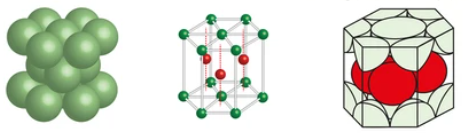
\includegraphics[width=0.5\linewidth]{Problem_2/Image/P2_I3.png}
     \caption{Hệ lục giác xếp chặt}
     \label{P2_I3}
\end{figure}

\Figref{P2_I3} biểu diễn mặt cắt ngang của một phần trong mạng tinh thể.

\begin{figure}[!ht]
    \centering

\begin{tikzpicture}[x=0.75pt,y=0.75pt,yscale=-1,xscale=1]
%uncomment if require: \path (0,347); %set diagram left start at 0, and has height of 347

%Shape: Regular Polygon [id:dp6255447637989042] 
\draw   (381.64,124.4) -- (368.9,146.47) -- (343.42,146.47) -- (330.68,124.4) -- (343.42,102.33) -- (368.9,102.33) -- cycle ;
%Shape: Circle [id:dp19888874912882015] 
\draw  [color={rgb, 255:red, 34; green, 141; blue, 36 }  ,draw opacity=1 ][fill={rgb, 255:red, 34; green, 141; blue, 36 }  ,fill opacity=1 ] (334.28,124.48) .. controls (334.28,112.44) and (344.04,102.68) .. (356.08,102.68) .. controls (368.12,102.68) and (377.88,112.44) .. (377.88,124.48) .. controls (377.88,136.52) and (368.12,146.28) .. (356.08,146.28) .. controls (344.04,146.28) and (334.28,136.52) .. (334.28,124.48) -- cycle ;
%Shape: Regular Polygon [id:dp9764763583068227] 
\draw   (342.84,146.4) -- (330.1,168.47) -- (304.62,168.47) -- (291.88,146.4) -- (304.62,124.33) -- (330.1,124.33) -- cycle ;
%Shape: Circle [id:dp5053963836368837] 
\draw  [color={rgb, 255:red, 34; green, 141; blue, 36 }  ,draw opacity=1 ][fill={rgb, 255:red, 34; green, 141; blue, 36 }  ,fill opacity=1 ] (295.48,146.48) .. controls (295.48,134.44) and (305.24,124.68) .. (317.28,124.68) .. controls (329.32,124.68) and (339.08,134.44) .. (339.08,146.48) .. controls (339.08,158.52) and (329.32,168.28) .. (317.28,168.28) .. controls (305.24,168.28) and (295.48,158.52) .. (295.48,146.48) -- cycle ;
%Shape: Regular Polygon [id:dp5886764579883312] 
\draw   (381.64,168.4) -- (368.9,190.47) -- (343.42,190.47) -- (330.68,168.4) -- (343.42,146.33) -- (368.9,146.33) -- cycle ;
%Shape: Circle [id:dp5631783623412631] 
\draw  [color={rgb, 255:red, 34; green, 141; blue, 36 }  ,draw opacity=1 ][fill={rgb, 255:red, 34; green, 141; blue, 36 }  ,fill opacity=1 ] (334.28,168.48) .. controls (334.28,156.44) and (344.04,146.68) .. (356.08,146.68) .. controls (368.12,146.68) and (377.88,156.44) .. (377.88,168.48) .. controls (377.88,180.52) and (368.12,190.28) .. (356.08,190.28) .. controls (344.04,190.28) and (334.28,180.52) .. (334.28,168.48) -- cycle ;
%Shape: Regular Polygon [id:dp9129386535407586] 
\draw   (420.04,146) -- (407.3,168.07) -- (381.82,168.07) -- (369.08,146) -- (381.82,123.93) -- (407.3,123.93) -- cycle ;
%Shape: Circle [id:dp5974572788947818] 
\draw  [color={rgb, 255:red, 34; green, 141; blue, 36 }  ,draw opacity=1 ][fill={rgb, 255:red, 34; green, 141; blue, 36 }  ,fill opacity=1 ] (372.68,146.08) .. controls (372.68,134.04) and (382.44,124.28) .. (394.48,124.28) .. controls (406.52,124.28) and (416.28,134.04) .. (416.28,146.08) .. controls (416.28,158.12) and (406.52,167.88) .. (394.48,167.88) .. controls (382.44,167.88) and (372.68,158.12) .. (372.68,146.08) -- cycle ;
%Shape: Regular Polygon [id:dp6661414486894639] 
\draw   (342.84,191.2) -- (330.1,213.27) -- (304.62,213.27) -- (291.88,191.2) -- (304.62,169.13) -- (330.1,169.13) -- cycle ;
%Shape: Circle [id:dp27399126763615] 
\draw  [color={rgb, 255:red, 34; green, 141; blue, 36 }  ,draw opacity=1 ][fill={rgb, 255:red, 34; green, 141; blue, 36 }  ,fill opacity=1 ] (295.48,191.28) .. controls (295.48,179.24) and (305.24,169.48) .. (317.28,169.48) .. controls (329.32,169.48) and (339.08,179.24) .. (339.08,191.28) .. controls (339.08,203.32) and (329.32,213.08) .. (317.28,213.08) .. controls (305.24,213.08) and (295.48,203.32) .. (295.48,191.28) -- cycle ;
%Shape: Regular Polygon [id:dp29268315893591157] 
\draw   (420.04,190.8) -- (407.3,212.87) -- (381.82,212.87) -- (369.08,190.8) -- (381.82,168.73) -- (407.3,168.73) -- cycle ;
%Shape: Circle [id:dp06073932786413472] 
\draw  [color={rgb, 255:red, 34; green, 141; blue, 36 }  ,draw opacity=1 ][fill={rgb, 255:red, 34; green, 141; blue, 36 }  ,fill opacity=1 ] (372.68,190.88) .. controls (372.68,178.84) and (382.44,169.08) .. (394.48,169.08) .. controls (406.52,169.08) and (416.28,178.84) .. (416.28,190.88) .. controls (416.28,202.92) and (406.52,212.68) .. (394.48,212.68) .. controls (382.44,212.68) and (372.68,202.92) .. (372.68,190.88) -- cycle ;
%Shape: Regular Polygon [id:dp03305034719229383] 
\draw   (382.04,212.8) -- (369.3,234.87) -- (343.82,234.87) -- (331.08,212.8) -- (343.82,190.73) -- (369.3,190.73) -- cycle ;
%Shape: Circle [id:dp2658805153093593] 
\draw  [color={rgb, 255:red, 34; green, 141; blue, 36 }  ,draw opacity=1 ][fill={rgb, 255:red, 34; green, 141; blue, 36 }  ,fill opacity=1 ] (334.68,212.88) .. controls (334.68,200.84) and (344.44,191.08) .. (356.48,191.08) .. controls (368.52,191.08) and (378.28,200.84) .. (378.28,212.88) .. controls (378.28,224.92) and (368.52,234.68) .. (356.48,234.68) .. controls (344.44,234.68) and (334.68,224.92) .. (334.68,212.88) -- cycle ;
%Shape: Regular Polygon [id:dp6205445172973503] 
\draw   (393.24,191.6) -- (380.5,213.67) -- (355.02,213.67) -- (342.28,191.6) -- (355.02,169.53) -- (380.5,169.53) -- cycle ;
%Shape: Circle [id:dp2865408738737726] 
\draw  [color={rgb, 255:red, 34; green, 141; blue, 36 }  ,draw opacity=1 ][fill={rgb, 255:red, 84; green, 190; blue, 85 }  ,fill opacity=1 ][dash pattern={on 4.5pt off 4.5pt}] (308.68,168.48) .. controls (308.68,156.44) and (318.44,146.68) .. (330.48,146.68) .. controls (342.52,146.68) and (352.28,156.44) .. (352.28,168.48) .. controls (352.28,180.52) and (342.52,190.28) .. (330.48,190.28) .. controls (318.44,190.28) and (308.68,180.52) .. (308.68,168.48) -- cycle ;
%Shape: Regular Polygon [id:dp07205505237456866] 
\draw   (394.04,147.2) -- (381.3,169.27) -- (355.82,169.27) -- (343.08,147.2) -- (355.82,125.13) -- (381.3,125.13) -- cycle ;
%Shape: Regular Polygon [id:dp010455195650463045] 
\draw   (355.24,168.8) -- (342.5,190.87) -- (317.02,190.87) -- (304.28,168.8) -- (317.02,146.73) -- (342.5,146.73) -- cycle ;
%Shape: Circle [id:dp8098844919275643] 
\draw  [color={rgb, 255:red, 34; green, 141; blue, 36 }  ,draw opacity=1 ][fill={rgb, 255:red, 84; green, 190; blue, 85 }  ,fill opacity=1 ][dash pattern={on 4.5pt off 4.5pt}] (345.88,191.28) .. controls (345.88,179.24) and (355.64,169.48) .. (367.68,169.48) .. controls (379.72,169.48) and (389.48,179.24) .. (389.48,191.28) .. controls (389.48,203.32) and (379.72,213.08) .. (367.68,213.08) .. controls (355.64,213.08) and (345.88,203.32) .. (345.88,191.28) -- cycle ;
%Shape: Circle [id:dp5549849514762719] 
\draw  [color={rgb, 255:red, 34; green, 141; blue, 36 }  ,draw opacity=1 ][fill={rgb, 255:red, 84; green, 190; blue, 85 }  ,fill opacity=1 ][dash pattern={on 4.5pt off 4.5pt}] (346.68,147.28) .. controls (346.68,135.24) and (356.44,125.48) .. (368.48,125.48) .. controls (380.52,125.48) and (390.28,135.24) .. (390.28,147.28) .. controls (390.28,159.32) and (380.52,169.08) .. (368.48,169.08) .. controls (356.44,169.08) and (346.68,159.32) .. (346.68,147.28) -- cycle ;
%Straight Lines [id:da26769465216326904] 
\draw    (313.24,162.36) -- (249.78,183.49) ;
\draw [shift={(247.88,184.12)}, rotate = 341.59] [color={rgb, 255:red, 0; green, 0; blue, 0 }  ][line width=0.75]    (10.93,-3.29) .. controls (6.95,-1.4) and (3.31,-0.3) .. (0,0) .. controls (3.31,0.3) and (6.95,1.4) .. (10.93,3.29)   ;
%Straight Lines [id:da4979225738352321] 
\draw    (404.44,133.52) -- (489.92,202.62) ;
\draw [shift={(491.48,203.88)}, rotate = 218.95] [color={rgb, 255:red, 0; green, 0; blue, 0 }  ][line width=0.75]    (10.93,-3.29) .. controls (6.95,-1.4) and (3.31,-0.3) .. (0,0) .. controls (3.31,0.3) and (6.95,1.4) .. (10.93,3.29)   ;

% Text Node
\draw (196.44,167.2) node [anchor=north west][inner sep=0.75pt]   [align=left] {lớp trên};
% Text Node
\draw (483.64,200.12) node [anchor=north west][inner sep=0.75pt]   [align=left] {lớp dưới};


\end{tikzpicture}
\caption{Hình ảnh của mặt cắt ngang}
\label{P2_tikz3}
\end{figure}

 Sử dụng \figref{P2_I2}:

\begin{enumerate}[label=(\alph*)]
\addtocounter{enumi}{3}
    \item Đánh giá tổng số liên kết bị gãy lúc này.
    \item Ước tính năng lượng liên kết và so sánh với phần trước.
    \item Tính phần trăm năng lượng va chạm được dùng để bẻ dãy các liên kết. So sánh với phần trước.
\end{enumerate}